\documentclass{article}
\usepackage{graphicx} % Required for inserting images
\usepackage{float}

\begin{document}
\linespread{1.5}
\section{Control}
\subsection{Plant Model Equations}
This section of the report will explain how the plant model equations are obtained. Followed by how these equations are implemented in MATLAB/Simulink \\

The plant model is a series of equations with multiple variables, which uses inputs, states, and parameters to get a certain output. 
For this project, the plant model is designed to take a height input the drone should hover at, paired with the inputs from the sensors, to achieve the desired hover height and stability.

\subsubsection{State Equations}
The drone possesses 6 degrees of freedom, enabling it to navigate in various directions and perform rotations. It can move along the X, Y, and Z axes, while also being capable of pitch (rotation around the Y axis), roll (rotation around the X axis), and yaw (rotation around the Z axis). We can identify the precise angle and position of the drone at any time by defining the axis of rotation and its accompanying state variables.
\cite{Ferry}

\begin{figure}[H]
\begin{center}
    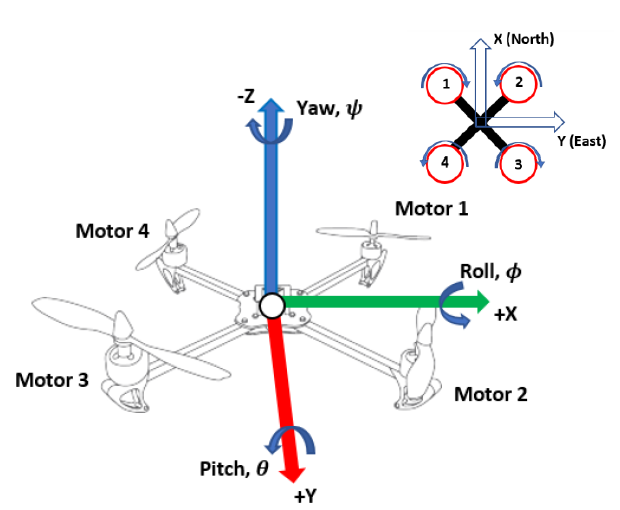
\includegraphics[scale =0.7]{images/drone directionals.png}
\end{center}
\caption{Quadcopter 'x' configuration}
\end{figure}

The drone's states include critical physical properties like as acceleration, velocity, and position, which are all detected by sensors. A gyroscope is used to record the angular changes of the drone. An accelerometer is a device that measures acceleration along the x, y, and z axes. Since the gyroscope drifts and the accelerator has measurement spikes when subjected to high acceleration, a complementary filter will be needed, which will be discussed in the “IMU” subsection. A dedicated infrared sensor is also used to measure distances in the z-direction, allowing for exact location information.

\begin{figure}[H]
\begin{center}
    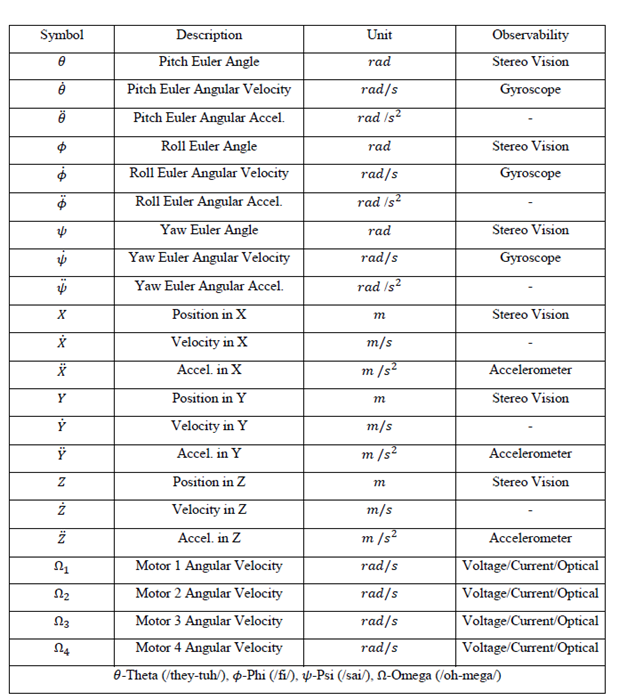
\includegraphics[scale =1]{images/State table.png}
\end{center}
\caption{State table}
\end{figure}

Before plant model equations can be generated, parameters for the drone need to be calculated. The parameters are what explains the drone mathematically and is an integral part of modelling the drone. The more accurate these values are the more realistic the plant model will be.
The parameters needed can be seen in the table below:\cite{Ferry}

\begin{figure}[H]
\begin{center}
    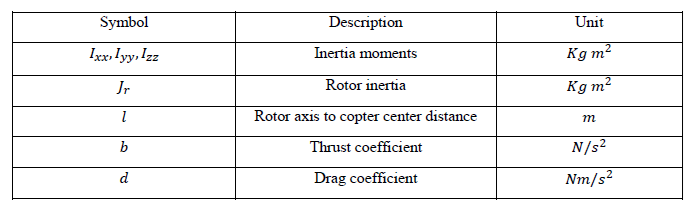
\includegraphics[scale =0.9]{images/parameter table.png}
\end{center}
\caption{State table}
\end{figure}

\subsubsection{Inertia Moments}
A moment of inertia is a constant value that explains the force/torque required to rotate an object in the direction of the moment. A desired angular velocity around a rotation axis can be found. The moments of inertia are found using estimation. If it is assumed that the drone is symmetrical in all axis, the moments of inertia can be found using parallel axis theorem to approximate the moments for each individual part of the drone in the x, y, z directions. For the calculations it’s assumed that the centre of mass for the drone is perfectly in the centre of the drone’s body.
The equations used for each individual part of the drone can be found in. \cite{Ferry}

For the approximation smaller electrical components were not considered, such as wires and mosfets, since their collective total weight is less than a gram, they are deemed negligible for the accuracy estimation.

\begin{figure}[H]
\begin{center}
   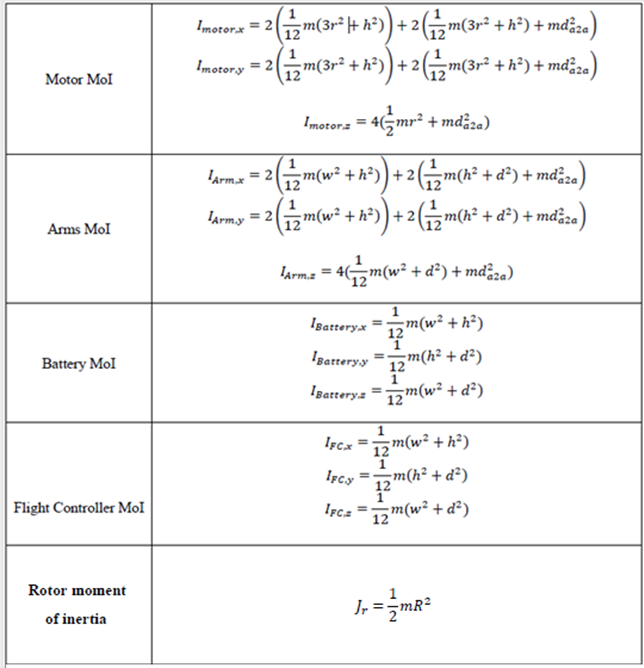
\includegraphics[scale =0.87]{images/inertia tables table.png}
\end{center}
\caption{Inertia moments equations}
\end{figure}

\begin{figure}[H]
\begin{center}
   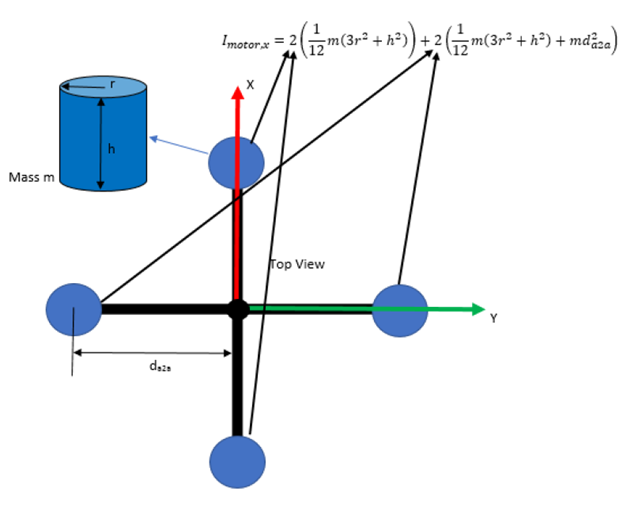
\includegraphics[scale =1]{images/Drone view inertiacalc.png}
\end{center}
\caption{Top view of quadcoptor}
\end{figure}

A mathematical document can be found in the appendix as “SPRO4math”. Which shows the detailed process of calculation. The mathematical equations are set up in maple, allowing quick changes to values in case a part is changed or removed. This feature proved useful since the weight estimate of the drone has changed rapidly over the course of the project period, as well as new components being added, which could then easily be integrated in the calculations.\\

\begin{figure}[H]
\begin{center}
   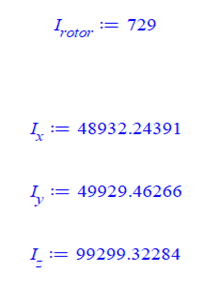
\includegraphics[scale =1]{images/Inertia moments.png}
\end{center}
\caption{Moments of inertia in the x, y, z axis, in $g*mm^2$ as calculated from equations, used in the final version of the quadcopter}
\end{figure}

\subsubsection{Characterization of Motor}
Some drone parameters can not be determined due to a lack of data concerning the motors used in the project. The motors are of a commercial product, but with no available data sheet. This means that motor constants and thrust coefficients needs to be determined through testing. Other motors within the same weight class were available, but those other alternatives did not provide the thrust desired compared to their weight, since the weight requirement set for the project is around 40 grams. For the same reason the motors currently in use are good, since they have a good thrust to weight ratio, with the caveat of not having a data sheet\\
The next part of the report is a small summary of the tests done to determine the data needed for the motors. The full reports concerning testing and acquiring these values can be found in the appendix. 
\begin{itemize}
    \item Thrust testing can be found in appendix "Motor Thrust Report"
    \item Motor constants testing can be found in appendix "Motor Testing"
\end{itemize}

\begin{figure}[H]
\begin{center}
   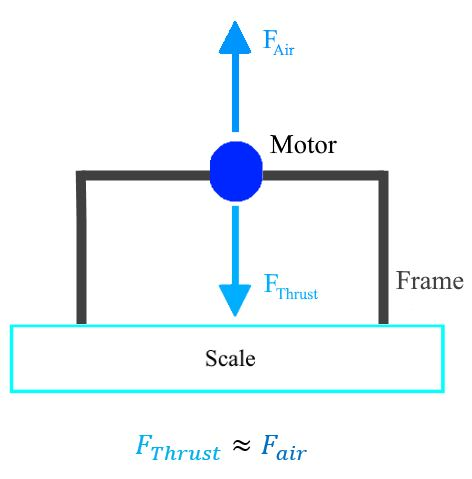
\includegraphics[scale =1]{images/Motor thrust 2.JPG}
\end{center}
\caption{Thrust testing setup}
\end{figure}

\subsubsection{Thrust testing}

For thrust testing the motor is placed in a frame on a scale to measure the change in weight when the motor is operating. The motor used had an operating voltage window of 0-4,2 volts, therefore the motor was tested between 1-4,2 volts incremented with 0,1 volts, and the weight change noted for each increment. Characterizing the motor yielded the results seen in the figure below.
As a general rule of thumb, provided by project supervisors, the motor's need to produce double the thrust of the total weight of the drone to operate ideally.
At maximum voltage level of the battery, a single motor produces 22.2 grams of thrust. In conclusion, at maximum voltage level the drone can ideally weigh 44.4 grams in total. The battery will slowly discharge meaning that it's impossible to always have max output, so it should be a little less than 44.4 grams in practice.

\begin{figure}[H]
\begin{center}
   \includegraphics[scale =1]{images/Graph thrust.JPG}
\end{center}
\caption{Thrust test data graphed}
\end{figure}

\subsubsection{Motor Constants, and Thrust Coefficient}
Motor constants relevant for this project include, “Motor velocity constant” ($K_v$) and “Motor torque constant” ($K_T$)
With a simple setup the motor's RPM can be tested proportionally to PWM. The motor was tested in 20 increments, using a photo sensor to measure RPM. Using the data from the test, we get the following result. \cite{MotorConstants}

\begin{figure}[H]
\begin{center}
   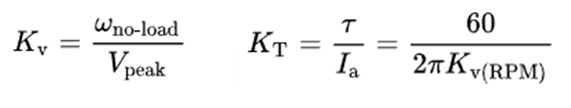
\includegraphics[scale =1]{images/Motor constants theory.png}
\end{center}
\caption{Equations used for calculating thrust- and velocity constants}
\end{figure}

\begin{figure}[H]
\begin{center}
   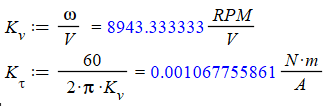
\includegraphics[scale =1.5]{images/Motor constants calc.png}
\end{center}
\caption{Motor Constants}
\end{figure}

Combining the two test data sets it is possible to determine the thrust coefficient of the motor. Using the graph from the thrust test the thrust can be calculated by taking the voltage drop over the motor. This thrust is then divided with the angular velocity to get the thrust coefficient ($TC=3.59E-05$).

The constants/coefficients are calculated around 3.0V inputs, which is the voltage needed to achieve the theoretical hover thrust. This is sensible since most of the time the drone will be operating around these values. 

\subsubsection{Environmental Forces}
The drone is very small, weighing only approximately 55grams as per requirement and with little surface area. Because of this, aerodynamic effects have been neglected for the modelling. Environmental forces mainly include but are not limited to wind resistance and liftoff turbulence.

\subsection{Plant Model Equations}
Now with the all the states and parameter defined, plant model equations can be generated. 
First, we will look at how the motors should operate together to move the quadcopter in the desired direction. A quadcopter can move in x and y directions using pitch and roll. When the quadcopter rotates around one of its axis, all the rotor blades will generate thrust at an angle, moving the drone in a direction. It is important to control the individual motors so the drone won’t tilt too much, causing it to flip in the air. On the picture below the different cases of directional movement for the quadcopter can be seen.  


\begin{figure}[H]
\begin{center}
   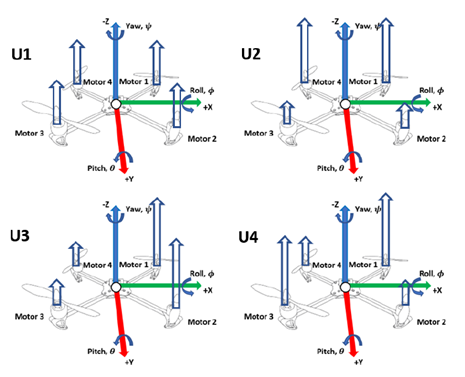
\includegraphics[scale =1]{images/thrust equations results.png}
\end{center}
\caption{Visual representation of thrust equations \cite{Ferry}}
\end{figure}

Here U1 is the general thrust behaviour, providing thrust equally and symmetrically to move only the Z axis. U2 creates a roll, thrusting the drone in the Y direction. U3 creates a pitch, thrusting the drone in the X direction. U4 increases the thrust for motors turning the same direction and decreases the thrust of the motors rotating the opposite direction, allowing the drone to rotate in the Z axis e.g., yaw due to non-symmetrical rotational forces created by the moments of the motors.  \cite{Ferry}

Each motors thrust is then defined as angular rotational speed to acquire the following equations.

\begin{figure}[H]
\begin{center}
   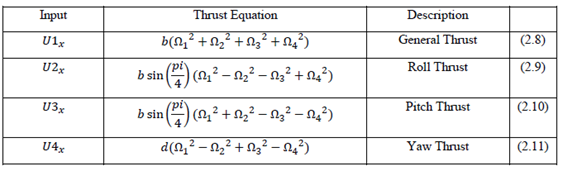
\includegraphics[scale =1]{images/thrust equations.png}
\end{center}
\caption{Thrust equations \cite{Ferry}}
\end{figure}

The plant equations for this project were gotten from one of the sources. For a more in depth description of how the plant equations are found see \cite{Ferry}
\begin{figure}[H]
\begin{center}
   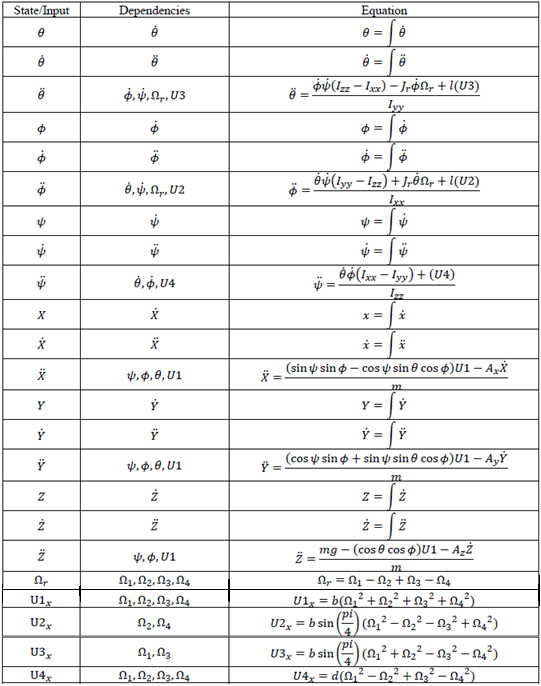
\includegraphics[scale =1]{images/plant equations.png}
\end{center}
\caption{Summary of plant equations \cite{Ferry}}
\end{figure}

\begin{figure}[H]
\begin{center}
   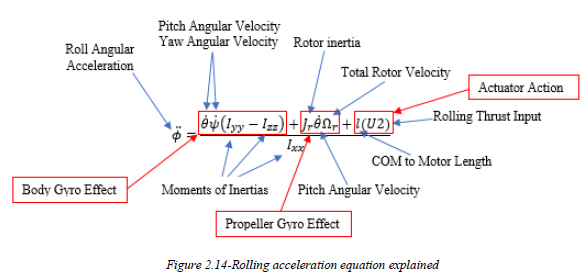
\includegraphics[scale =1]{images/plant equation example.png}
\end{center}
\caption{Example of plant equation for phi. \cite{Ferry}}
\end{figure}

Body gyroscopic effects from changes in the quadcopter orientation.
Propeller gyroscopic effects from propeller rotation and angle/orientation
Actuation action forces produced by the rotors/propellers.

\subsection{SIMULINK/Matlab Implementation}
To make the Simulink model the thrust equations must be transferred into the program using the angular speed as inputs and the motor parameters. Below we see the thrust equations in Simulink with the inputs on the left and outputs on the right. (The outputs are U1, U2, U3, and U4, as well as Omega) In SIMULINK the math is done using “blocks”, the addition and subtraction is performed first, and then the next blocks take the product. Essentially the math is converted using blocks in SIMULINK.

\begin{figure}[H]
\begin{center}
   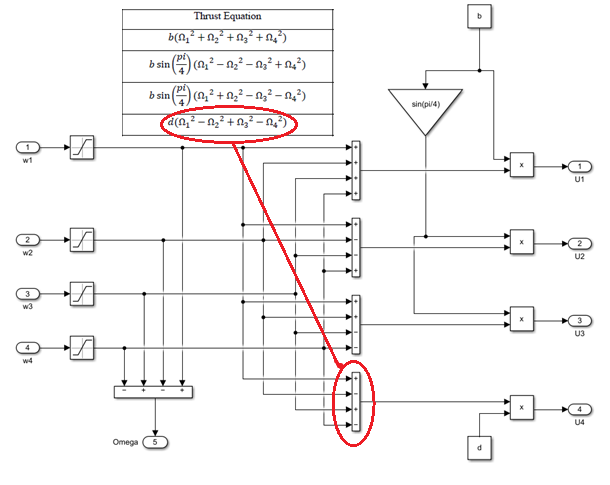
\includegraphics[scale =1]{images/thrust equation in simulink.png}
\end{center}
\caption{Thrust equations in SIMULINK}
\end{figure}

The rest of plant equations are then also transferred to SIMULINK using the same process, using blocks to represent the math. The next part of the plant takes the thrust equations as an input to calculate theta, phi, and psi, for position, velocity, and acceleration. \\

Below is an example for the equation of phi double dot. We use the thrust equations and feedback together with the drone parameters to get the result. Since all the equations need feedback from the other plant equations, an initial value must be set. It makes sense to make the initial value 0 since we haven’t moved yet and there has been no change in any direction or angle. Throughout the flight the drone will then fill out the theta, phi, and psi values using the censors to determine the change in position. For example, if the drone is slanted a bit in the direction of motor 4 and 1, the drone will have a change in the roll aka phi value. The censor will detect the magnitude of this change, and U2 will increase to give more thrust to those motors to stabilize. Thrust is increased proportionally to smoothing the stabilization. 

\begin{figure}[H]
\begin{center}
   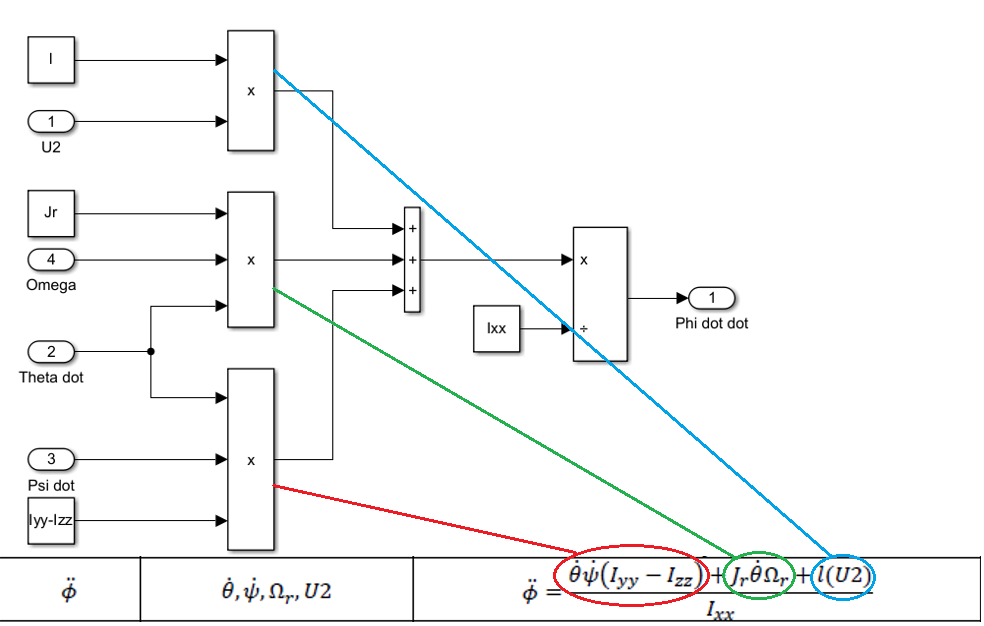
\includegraphics[scale =0.7]{images/plant equation phi example.png}
\end{center}
\caption{Plant equation for phi double dot}
\end{figure}

\begin{figure}[H]
\begin{center}
   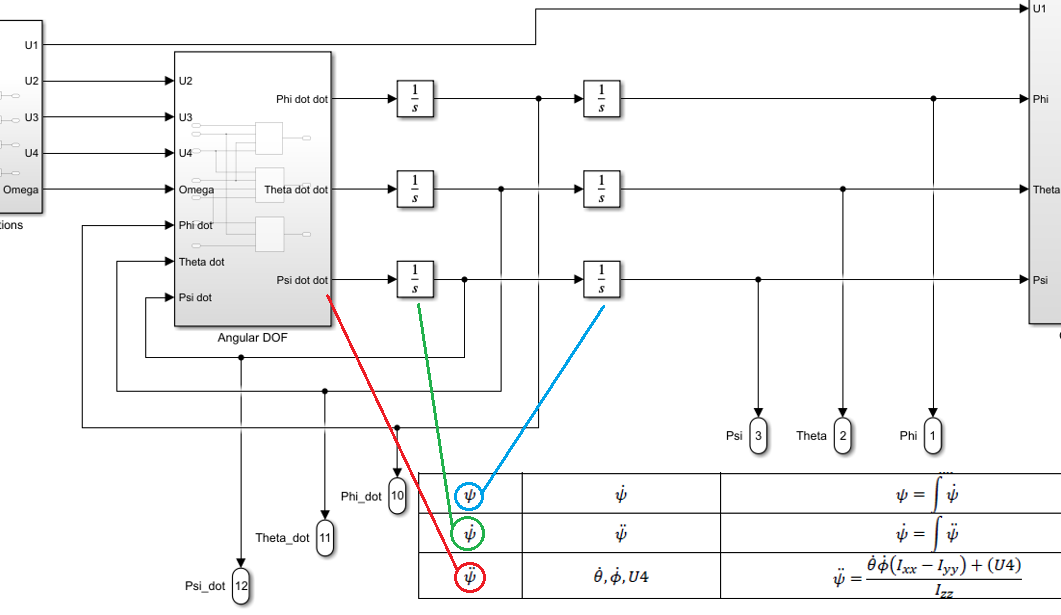
\includegraphics[scale =0.6]{images/plant pic1.png}
\end{center}
\caption{Angular equations overview example}
\end{figure}

To finish out the plant, the X, Y, and Z values for acceleration, velocity, and position are calculated using the values from theta, phi, and psi, these equations rely on feedback from each other in the same way that angles do, and use the same principles when it comes to determining the initial value. 

\begin{figure}[H]
   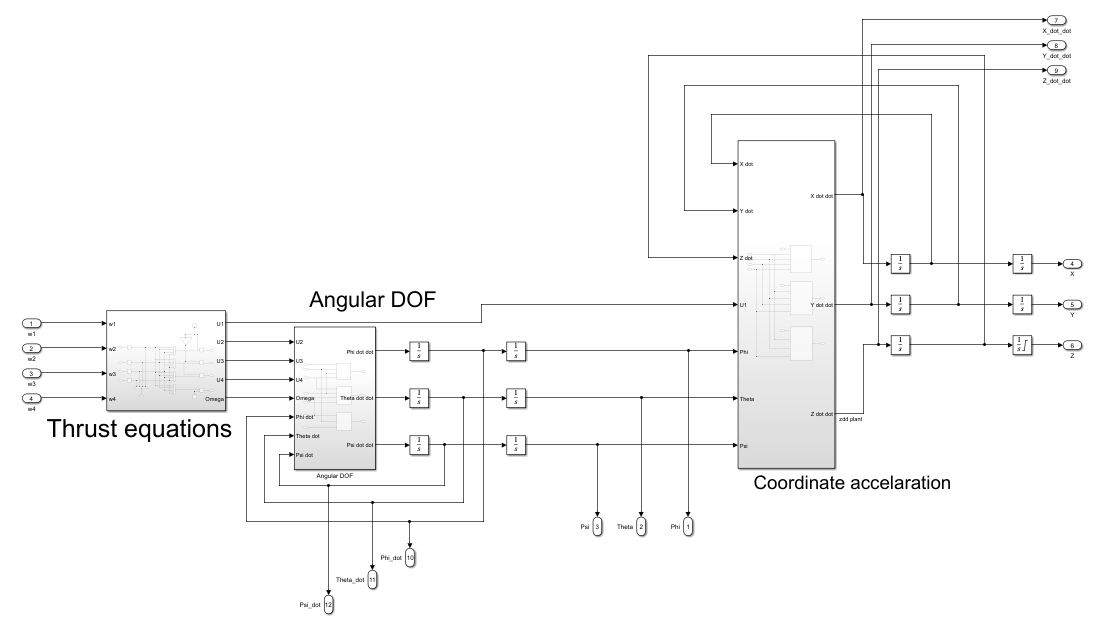
\includegraphics[scale =0.6]{images/Plant overview.png}
\caption{Plant overview in SIMULINK}
\end{figure}

\bibliographystyle{plain}
\bibliography{sources}
\end{document}
